\section{Recursão}

\begin{frame}
	\begin{block}{Recursão}
		\begin{itemize}
			\item O que é recursão? Uma função que chama ela mesma diversas vezes até convergir em um caso básico do problema, de solução simples. Após atingir esse caso, ela combina todos os resultados intermediários até retornar a solução do problema.
			
			\item É um paradigma computacional muito poderoso, permite resolver problemas de forma simples. Programas recursivos tem uma tendência de serem menores que sua abordagens iterativas.
			
			\item Está relacionada com conceito de indução matemática.
		\end{itemize}
	\end{block}
\end{frame}


\begin{frame}
	\begin{block}{Indução matemática}
		\begin{itemize}
			\item Indução matemática é uma técnica matemática para provar asserções sobre números naturais

			\item Dado um teorema $T$ com parâmetro $N$, que é um número natural. Precisamos provar que $T$ é válido.
			
			\item Usando indução matemática fazemos o seguinte procedimento:
			
			\item Provamos $T$ para $n = 1$ (chamado caso base)
			
			\item Para todo $T$ onde $N > 1$, se T é válido para $n-1$ então é válido para $N$ (passo indutivo)
		\end{itemize}
	\end{block}
\end{frame}


\begin{frame}
	\begin{block}{Indução matemática}
		\begin{itemize}
			\item Por que isso funciona? Por que apenas essas duas condições são suficientes?
			
			\item Simples, as condições 1 e 2 implicam que $T$ é válido para $n = 2 \ldots$	
			
			\item Pela condição 2, se for válido para $2$ será para $3 \ldots$ e assim sucessivamente.
		\end{itemize}
	\end{block}
\end{frame}

\begin{frame}
	\begin{block}{Indução matemática}
		\begin{itemize}
			\item Um exemplo matemático, a soma dos n primeiros números naturais n, pode ser escrita como: S(n) = 1+2+...+n. Sabemos que isso é a soma de uma PA com r = 1, como provar que a soma desses números é dada pela fórmula fechada: S(n) = n*(n+1)/2 ?
			
			\item Podemos usar indução!
			
			\item Passo base: n = 1 S(1) = 1 (trivial)
		\end{itemize}
	\end{block}
\end{frame}

\begin{frame}
	\begin{block}{Indução matemática}
		\begin{itemize}
			\item Passo Indutivo: 
		\end{itemize}
		\begin{eqnarray}
				S(n) = S(n-1) + n \Leftrightarrow \\
				((n-1) *(n-1+1) )/2 + n \Leftrightarrow \\
				n*(n+1) / 2
		\end{eqnarray}
		\begin{itemize}
			\item A partir da hipótese indutiva com parâmetro n-1 (fórmula fechada) chegamos em n provando por indução que funciona
		\end{itemize}
	\end{block}
\end{frame}


\begin{frame}
	\begin{block}{Indução matemática - Exercício}
		\begin{itemize}
			\item Como multiplicar dois números sem usar o operador de multiplicação? Programar a versão iterativa e a recursiva...
		\end{itemize}
	\end{block}
\end{frame}

\begin{frame}
	\begin{block}{Indução matemática - Exercício}
		\begin{itemize}
			\item A sequência de Fibonacci pode ser escrita como:

			\item $F(n)$  se $n <= 1$ então retorne $n$
			\item caso contrário$f(n-1) + f(n-2)$
			
			\item Vamos programar esse algoritmo....
		\end{itemize}
	\end{block}
\end{frame}

\begin{frame}
	\begin{block}{Indução matemática}
		\begin{itemize}
			\item Uma analogia usada para compreender recursão são as bonecas russas matrioskas
		\end{itemize}
		 \begin{figure}[!htb]
			\centering	  				
			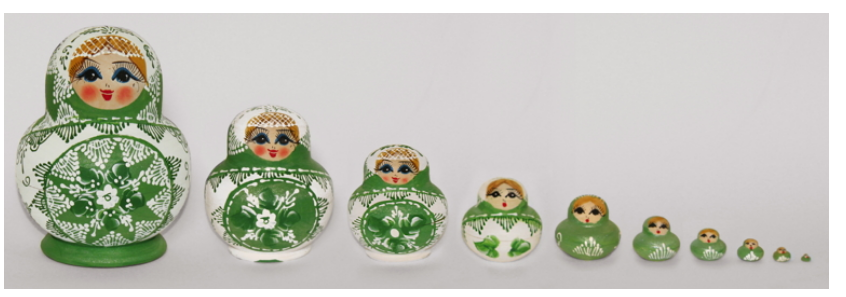
\includegraphics[height=5cm, width = 9cm]{./pic/nmatrioskas.png}
			\caption{Bonecas Matrioskas \cite{KHAN}}
			\label{fig_matrioskas}
		\end{figure}
	\end{block}
\end{frame}

\begin{frame}
	\begin{block}{Indução matemática "Forte"}
		\begin{itemize}
			\item Indução forte é uma estratégia parecida com indução fraca mas que origina algoritmos baseados em divisão e conquista.

			\item Novamente devemos provar o caso base:
			
			\item $N = 1$
			
			\item Mas agora, ao invés de provar para $n-1$ vamos provar que a hipótese é válida para qualquer $k<n$
		\end{itemize}
	\end{block}
\end{frame}

\begin{frame}
	\begin{block}{Indução matemática "Forte"}
		\begin{itemize}
			\item Citar algoritmo de exponenciação por indução forte

			\item $N = 0$ então $exp(a,0) = 1$ (caso base)
			
			\item Passo indutivo, sei calcular $exp(a,piso(n/2))$
			
			\item O cálculo seria: se $n\%2 = 0$ então $exp(a,piso(n/2))^2$
			\item  se $n\% 2 = 1$ então $exp(a,piso(n/2))^2$
			
			\item Explicar no quadro e programar!
		\end{itemize}
	\end{block}
\end{frame}

\begin{frame}
	\begin{block}{Tribonacci}
		\begin{itemize}
			\item A sequencia de Tribonacci é muito parecida com a série de Fibonacci. A diferença é que cada elemento é a soma dos três anteriores.

			\item Mostrar no quadro e programar com os alunos
		\end{itemize}
	\end{block}
\end{frame}